\documentclass[25pt, a0paper, portrait]{tikzposter}
\usepackage[utf8]{inputenc}
\renewcommand{\familydefault}{\sfdefault}   % sans serif font for better readibility

\title{\parbox{0.75\linewidth}{\centering Position Control of Parallel Combinations of Soft Actuators}}
% \title{Position Control of Parallel Combinations of Soft Actuators}
\author{Daniel Bruder, Audrey Sedal, Ram Vasudevan, C. David Remy}
% \date{\today}
\institute{University of Michigan}

\usepackage{blindtext}
\usepackage{comment}
\usetikzlibrary{calc}

\usetheme{Default}
\usebackgroundstyle{Empty}
\usetitlestyle{Empty}
\useblockstyle[roundedcorners=8]{Default} % Can use this line to change the stile of blocks for entire document
\useinnerblockstyle{Empty}


% BEGINNING OF DOCUMENT-------------------------------------------------------------------------------------
\begin{document}

\maketitle

% Put logos in the the top corners
\node[anchor=west] at (TP@title.west) {
\includegraphics[width=0.125\linewidth]{images/UMlogo.eps}};
\node[anchor=east] at (TP@title.east) (ROAHM) {
\includegraphics[width=0.125\linewidth]{images/ROAHMLABicon.pdf}};
\node[anchor=south] at (ROAHM.north) (RAM) {
\includegraphics[width=0.125\linewidth]{images/RAMlogo.pdf}};
\node[anchor=north] at (ROAHM.south) (CSDL) {
\includegraphics[width=0.125\linewidth]{images/csdl_logo.pdf}};


\begin{columns}

\column{0.5}

% Block 1 - Motivation
\block{Motivation}{Text and more text}

% Block 2 - Modeling
\block{Modeling}{\blindtext}

% Block 3 - Experiment
\block{Model was validated experimentally}{
    \begin{minipage}[c]{0.65\linewidth}
        \centering
        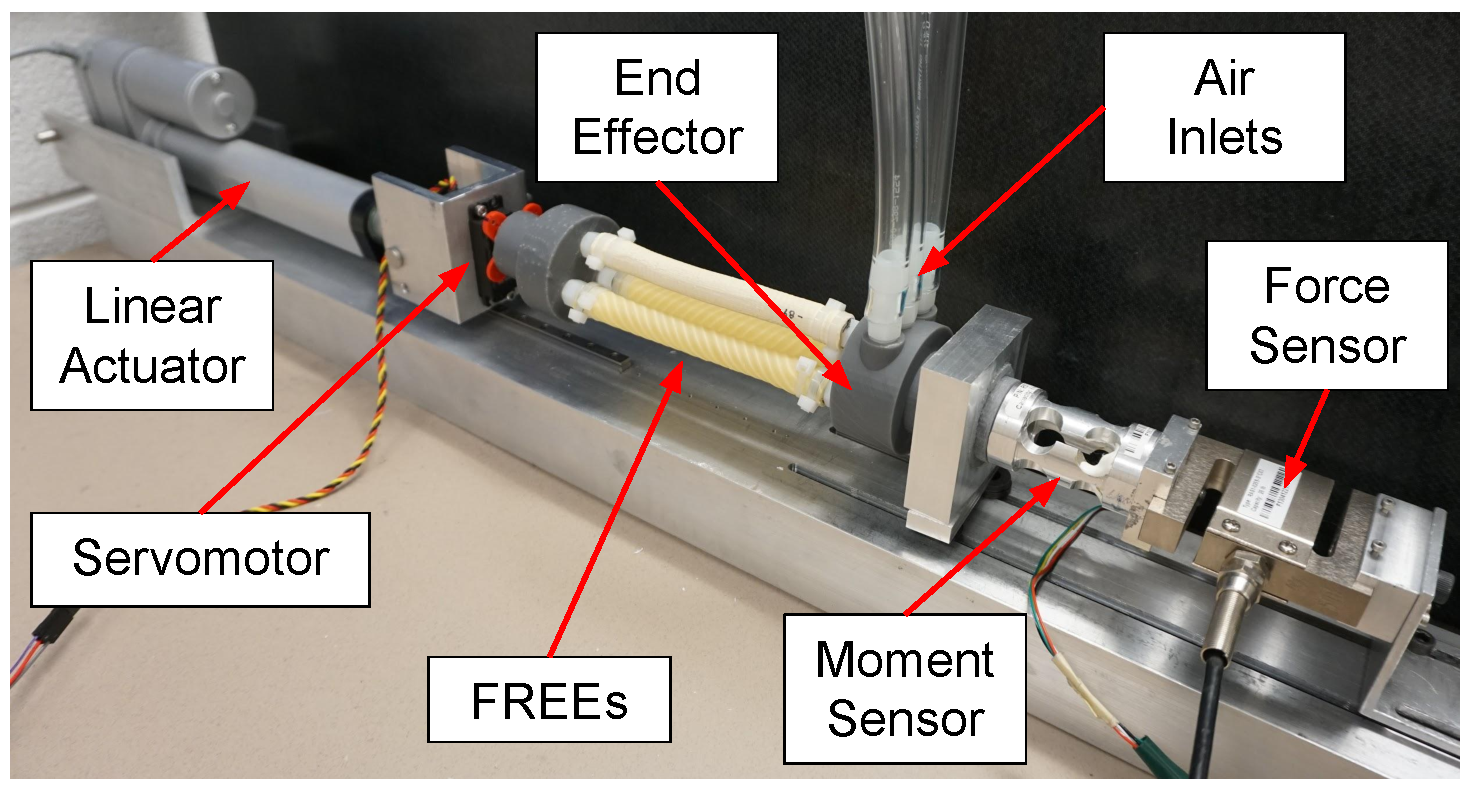
\includegraphics[width=\linewidth]{images/rig_labeled.pdf}
    \end{minipage}
    \hspace{10pt}
    \begin{minipage}[c]{0.3\linewidth}
        \centering
        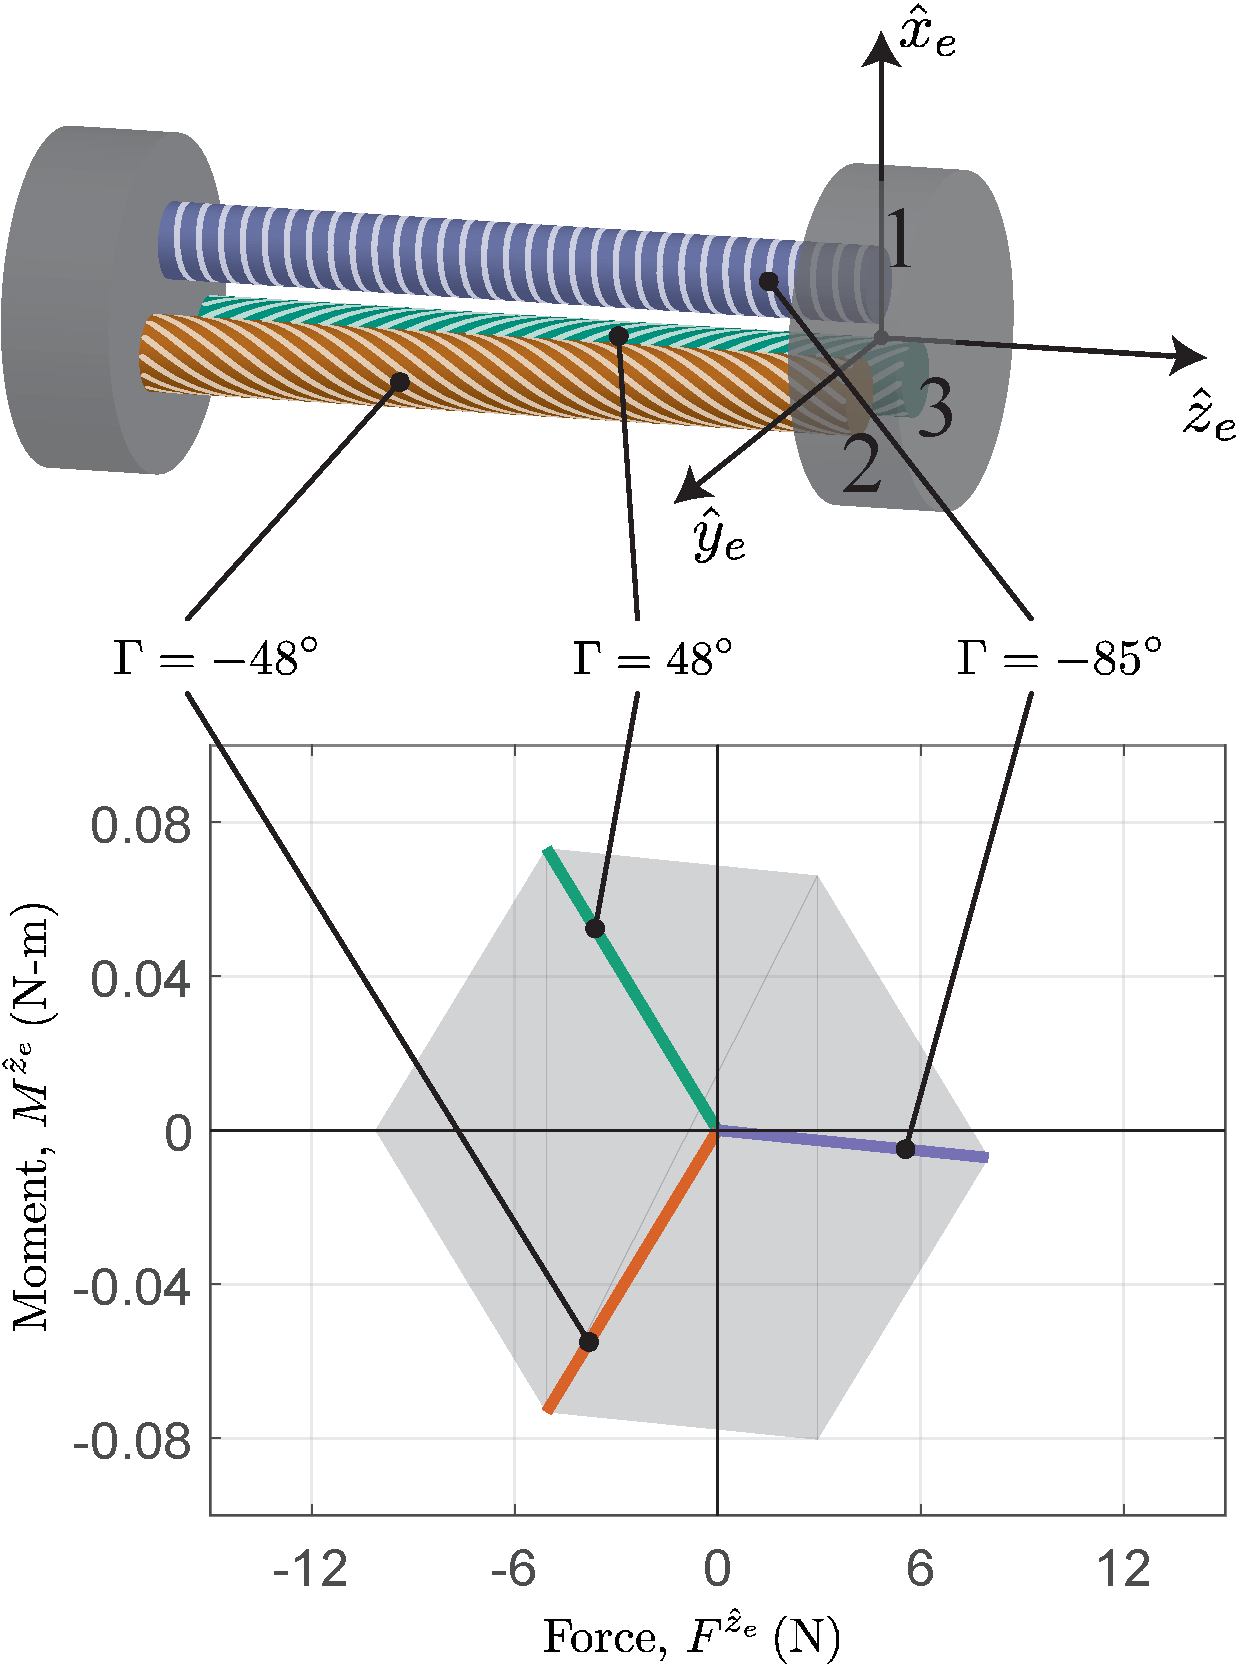
\includegraphics[width=\linewidth]{images/rigDiagram_wlabels10.pdf}
    \end{minipage}
}
    
\column{0.5}

% Block 4 - Applications
\block{Applications}{
    \begin{minipage}[c]{0.5\linewidth}
        \centering
        
\includegraphics[width=\linewidth]{images/UMlogo.eps}
    \end{minipage} %
    \begin{minipage}[c]{0.5\linewidth}
        \centering
        
\includegraphics[width=\linewidth]{images/csdl_logo.pdf}
    \end{minipage}
    
    \begin{minipage}[c]{\linewidth}
        \centering
        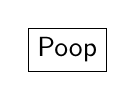
\begin{tikzpicture}
            \node[anchor=center, draw] at (0,0) (poopnode) {Poop};
        \end{tikzpicture}
    \end{minipage}
}

% Block 5 - Control
\block{Control}{
    \begin{minipage}[c]{\linewidth}
    \centering
    \begin{tikzpicture}
        \node[anchor=center] at (0,0) (testnode) {
\includegraphics[width=0.2\linewidth]{images/UMlogo.eps}};
        \node[anchor=center, draw] at (testnode.south east) (poopnode2) {Poop!!!};
    \end{tikzpicture}
    \end{minipage}
}

% Block 6 - References
\block{References}{\blindtext}
    
\end{columns}



\end{document}







%% EXTRA STUFF I MIGHT FIND USEFUL %%----------------------------------------------------------------

    % \note[
    %     targetoffsetx=-9cm, 
    %     targetoffsety=-6.5cm, 
    %     width=0.5\linewidth
    %     ]
    %     {e-mail \texttt{sharelatex@sharelatex.com}}
    
% \begin{columns}
%     \column{0.5}
%     \block{A figure}
%     {
%         \begin{tikzfigure}
%             
\includegraphics[width=0.4\textwidth]{images/lion-logo.png}
%         \end{tikzfigure}
%     }
%     \column{0.5}
%     \block{Description of the figure}{\blindtext}
% \end{columns}

% \begin{subcolumns}
%     \subcolumn{0.27} \block{1}{First block.} \block{2}{Second block}
%     \subcolumn{0.4} \block{Sub-columns}{Sample subblocks\\Second subcolumn}
%     \subcolumn{0.33} \block{4}{Fourth} \block{}{Final Subcolumn block}
% \end{subcolumns}